\documentclass{article}

% if you need to pass options to natbib, use, e.g.:
\PassOptionsToPackage{numbers, compress}{natbib}
% before loading neurips_2019

% ready for submission
% \usepackage{neurips_2019}

% to compile a preprint version, e.g., for submission to arXiv, add add the
% [preprint] option:
%     \usepackage[preprint]{neurips_2019}

% to compile a camera-ready version, add the [final] option, e.g.:
\usepackage[final]{finalreport} 
\usepackage{xcolor}
\usepackage{enumitem}
% to avoid loading the natbib package, add option nonatbib:
%     \usepackage[nonatbib]{neurips_2019}

\usepackage[utf8]{inputenc} % allow utf-8 input
\usepackage[T1]{fontenc}    % use 8-bit T1 fonts
\usepackage{hyperref}       % hyperlinks
\usepackage{url}            % simple URL typesetting
\usepackage{booktabs}       % professional-quality tables
\usepackage{amsfonts}       % blackboard math symbols
\usepackage{nicefrac}       % compact symbols for 1/2, etc.
\usepackage{microtype}      % microtypography
\usepackage{amsmath}
\usepackage{caption}
\usepackage{subcaption}
\usepackage{mathtools}
\usepackage{amssymb}
\usepackage[ruled,linesnumbered]{algorithm2e}
\usepackage{multirow}
\usepackage[toc,page]{appendix}

\newcommand{\shellcmd}[1]{\\\indent\indent\texttt{\footnotesize\$ #1}\\}
\newcommand{\pythoncmd}[1]{\\\indent\indent\texttt{\footnotesize>{}>{}> #1}\\}

\usepackage{xcolor}
\hypersetup{
    colorlinks,
    linkcolor={red!50!black},
    citecolor={blue!50!black},
    urlcolor={blue!80!black}
}

\title{Gibbs Sampler for Infinite Latent Feature Models}

% The \author macro works with any number of authors. There are two commands
% used to separate the names and addresses of multiple authors: \And and \AND.
%
% Using \And between authors leaves it to LaTeX to determine where to break the
% lines. Using \AND forces a line break at that point. So, if LaTeX puts 3 of 4
% authors names on the first line, and the last on the second line, try using
% \AND instead of \And before the third author name.

\author{%
  Bo Liu \\
  Department of Statistical Science\\
  Duke University\\
  Durham, NC 27705 \\
  \texttt{bl226@duke.edu} \\
  \And
  Linlin Li \\
  Department of Statistical Science\\
  Duke University\\
  Durham, NC 27705 \\
  \texttt{linlin.li434@duke.edu} \\
  % examples of more authors
  % \And
  % Coauthor \\
  % Affiliation \\
  % Address \\
  % \texttt{email} \\
  % \AND
  % Coauthor \\
  % Affiliation \\
  % Address \\
  % \texttt{email} \\
  % \And
  % Coauthor \\
  % Affiliation \\
  % Address \\
  % \texttt{email} \\
  % \And
  % Coauthor \\
  % Affiliation \\
  % Address \\
  % \texttt{email} \\
}


\begin{document}

\maketitle

\begin{abstract}
  The Indian buffet process is a generative process that results in a probability distribution over equivalence classes of binary matrices with an unbounded number of columns. This distribution is often used as a prior in infinite latent feature models where the objects are represented by a potentially infinite array of features. In this paper, we introduce an implementation on a Gibbs sampler for inference in this model, perform optimizations and correctness check, and apply it to simulated and real datasets. Comparison with existing algorithms shows that a noticeable gain in performance is achieved.
\end{abstract}

\paragraph{Key words:} Indian buffet process, binary matrix, infinite latent feature model, Gibbs sampler.

\section{Background}

Clustering is a set of methods that have been extensively studied and used in unsupervised learning since its first appearance in 1954 \citep{caron2018deep}. A large number of these methods assume that each observation belongs to one of some mutually exclusive clusters and attempt to classify the observations, although the classification can be deterministic (e.g. K means \citep{steinhaus1956division, lloyd1982least}) or probabilistic (e.g. Latent Dirichlet Allocation \citep{blei2003latent}). However, many datasets do not intrinsically satisfy the assumption. Instead, they share multiple latent features and each observation contains a subset of these features. An example is in image detection where the aim is to identify and position items in images \citep{zhang2018multilabel}. Multi-labeled data are also common in recommendation system, where each item is related to multiple tags \citep{zheng2014context}.

All of these methods confront the critical challenge to determine how many latent features are necessary to model the hidden structure beyond the data. Usually, models with various number of latent features are tested and the optimal dimensionality is chosen based upon some metric on complexity or generalization error. In a Bayesian context, the dimensionality is controlled by both the prior belief and the data. Under this setting, the number of latent features can be infinite, and the data only reveal a finite subset of these features \citep{rasmussen2001occam}, such as Dirichlet process mixture models \citep{antoniak1974mixtures}. In a Dirichlet process mixture model, each object belongs to one of the latent classes, and each latent class defines a distribution over all latent features. The prior distribution of each class, which is a Dirichlet Process, is discrete with probability 1, but takes non-zero probability at infinite values \citep{teh2010dirichlet}, assuring Dirichlet process mixture models to have infinite underlying features \citep{rasmussen2000infinite}. Beta process can be the prior distribution on the probability of each latent feature if each observation has multiple features \citep{JMLR:v12:griffiths11a}. Similarly, such models also have infinite dimensionality in the latent features.

Dirichlet and Beta process have been studied as priors in non-parametric Bayesian modelling. Both processes can be reparameterized with stick breaking processes \citep{broderick2012beta, paisley2011stick}. Moreover, these processes can be specified by sequential processes, respectively, the Chinese restaurant process \citep{griffiths2004hierarchical} and the Indian Buffet process \citep{thibaux2007hierarchical}. 

\citet{ghahramani2006infinite} describes how Indian buffet process can be used as a prior in statistical models where each object is represented by a subset of infinite features \citep[also see][]{griffiths2005infinite}. In this paper, we implement a Gibbs sampler which generates Dirichlet process as a prior and samples from the posterior distribution. 

We describe the algorithm in Section \ref{sec::description} and introduce the optimization on our implementation in Section \ref{sec::optimization}. In Sections \ref{sec::simulation} and \ref{sec::realdata} we show how the algorithm can be applied to extract latent features in an image. The algorithm performs well with both simulated data and real data. We compare our implementation with other similar ones in Section \ref{sec::comparison}, and conclude in Section \ref{sec::discussion}. 


\section{Description of the algorithm}\label{sec::description}

We implemented a Gibbs sampler on a linear-Gaussian binary latent feature model, where each observation is assumed to contain some of underlying features. The prior on the feature matrix is Gaussian, and the prior on the (binary) indicator matrix is a Dirichlet process. Our sampler is able to sample the indicators and the features from their posterior distributions.

\subsection{Notations and conventions}

Suppose $\mathbf{X}$ is an $N\times D$ matrix of objects, each row being an observation consisting of $D$ components. The underlying latent features, which also lie in $\mathbb{R}^D$, are denoted as $\mathbf{A} \in \mathbb{R}^{K\times D}$, $K$ being the total number of features revealed by the data. Note that $K$ may vary during the sampling and there is a prior on it. $\mathbf{Z}$ is an $N\times K$ indicator matrix consisting of $0$'s and $1$'s, indicating whether an observation contains some certain feature.

Any vector without subscripts or superscripts should be considered a column vector unless specified. For any matrix $\mathbf{X}$, the $i$-th row is denoted as $\boldsymbol{x}_{i\cdot}$ and the $j$-th column is denoted as $\boldsymbol{x}_{\cdot j}$. The $(i,j)$-th entry of $\mathbf{X}$ is denoted as $x_{ij}$. $\boldsymbol{e}_k$ is a column vector with all entries being 0 except the $k$-th entry being 1. $\mathbf{E}_{ij}$ is a matrix with all entries  being 0 except the $(i,j)$-th entry being 1. $\mathbf{I}$ is the identity matrix.

For Gibbs sampler, we use a number in bracket to indicate a sample in a specific iteration, (e.g. $\mathbf{Z}^{(t)}$ is the sampled matrix $\mathbf{Z}$ in the $t$-th iteration).

\subsection{Priors and assumptions}
\begin{itemize}
  \item We define an Indian buffet process on the prior of $\mathbf{Z}$. The Indian buffet process scheme is introduced by \citet[Sec 2.4]{griffiths2005infinite}. Using $K_1^{(i)}$ to indicate the number of new dishes sampled by the $i$-th customer, the probability of any particular matrix being produce by the IBP is \begin{equation}P(\mathbf{Z}\mid\alpha) = \frac{\alpha^{K}}{\prod_{i=1}^NK_1^{(i)}!}\exp\{-\alpha H_N\}\prod_{k=1}^K\frac{(N - m_k)!(m_k - 1)!}{N!},\end{equation}
  where $m_k = \sum_{i=1}^N z_{ik}$ is the number of objects possessing feature $k$, and \begin{equation}H_N = \sum_{n = 1}^N\frac{1}{n}.\end{equation}
  \item The feature matrix has a Gaussian prior \begin{equation}\mathbf{A}\mid K, \sigma_A\sim \mathcal{MN}(\mathbf{O}_{K\times D}, \mathbf{I}_K, \sigma_A^2\mathbf{I}_D).\end{equation}
  \item Given $\mathbf{Z}$ and $\mathbf{A}$, the distribution of $\mathbf{X}$ is Gaussian \begin{equation}\mathbf{X}\mid \mathbf{Z}, \mathbf{A}, \sigma_X \sim \mathcal{MN}(\mathbf{ZA}, \mathbf{I}_N, \sigma_X^2\mathbf{I}_D).\end{equation}
  \item The prior distribution of $\alpha$, $\sigma_A$ and $\sigma_X$ are gamma distributions.
  \begin{equation}
  \begin{aligned}
    \alpha &\sim \mathcal{G}(\alpha^a, \alpha^b);\\
    \sigma_X &\sim \mathcal{G}^{-1}(\sigma_X^a,\sigma_X^b);\\
    \sigma_A &\sim \mathcal{G}^{-1}(\sigma_A^a, \sigma_A^b).
  \end{aligned}
  \end{equation}
  \item If a column of $\mathbf{Z}$ are all $0$'s, this column as well as the corresponding row in $\mathbf{A}$ are removed, as no entries in this column will be assigned $1$ in the Gibbs sampler.
\end{itemize}

\subsection{Full conditionals}
  \citet{griffiths2005infinite} noticed that $\mathbf{A}$ can be integrated out, so there is no need to update $\mathbf{A}$ each step.
  \begin{multline}
    p(\mathbf{X}\mid \mathbf{Z}, \sigma_X, \sigma_A) = \frac{1}{(2\pi)^{ND/2}\sigma_X^{(N-K)D}\sigma_A^{KD}|{\mathbf{Z}}^{\mathrm{T}}\mathbf{Z}+\frac{\sigma_X^2}{\sigma_A^2}\mathbf{I}|^{D/2}} \\
    \exp\left\{-\frac{1}{2\sigma_X^2}\mathrm{tr}({\mathbf{X}}^{\mathrm{T}}(\mathbf{I}-\mathbf{Z}({\mathbf{Z}}^{\mathrm{T}}\mathbf{Z}+\frac{\sigma_X^2}{\sigma_A^2}\mathbf{I})^{-1}{\mathbf{Z}}^{\mathrm{T}})\mathbf{X})\right\}.
  \end{multline}
\begin{itemize}
  \item Full conditional for $\mathbf{Z}$:
  
  As the dimension of $\mathbf{Z}$ may change through the sampling, we need to find the full conditional for both the original and the (potential) additional columns of $\mathbf{Z}$.
  \begin{itemize}
    \item For $k = 1, \cdots, K$, \begin{equation}P(z_{ik}\mid \mathbf{X},\mathbf{Z}_{-(i,k)}, \sigma_X, \sigma_A)\propto p(\mathbf{X}\mid \mathbf{Z}, \sigma_X, \sigma_A)P(z_{ik}\mid \boldsymbol{z}_{-i, k}),\end{equation}
    where $P(z_{ik} = 1\mid\boldsymbol{z}_{-i, k}) = \frac{m_{-i, k}}{N}$.

    $m_{-i,k}$ denotes the number of objects possessing feature $k$, excluding $i$.
    \item There might be $K_i^\text{new}$ columns added to $\mathbf{Z}$, each additional column being $\boldsymbol{e}_i$.
    \begin{equation}P(K_i^\text{new}\mid \mathbf{X},\mathbf{Z},\sigma_X,\sigma_A,\alpha) \propto p(\mathbf{X}\mid \mathbf{Z}_{i,K_i^\text{new}}^{+},\sigma_X,\sigma_A)P(K_i^\text{new}\mid\alpha),\end{equation}
    where $K_i^\text{new}\mid \alpha \sim \mathrm{Possion}(\alpha/N)$, 
    \begin{equation}\mathbf{Z}_{i,K_i^\text{new}}^+ = \begin{pmatrix}
      \mathbf{Z}, \smash{\underbrace{\boldsymbol{e}_i, \cdots, \boldsymbol{e}_i}_{K_i^\mathrm{new}\text{ columns}}}
    \end{pmatrix}.\end{equation}
  \end{itemize}
  \item Full conditional for $\alpha$:
  \begin{equation}\alpha\mid \mathbf{Z}\sim \mathcal{G}(\alpha^a + K, \alpha^b + H_N).\end{equation}
  \item Full conditional for $\sigma_X$ and $\sigma_A$:
  \begin{equation}
  \begin{aligned}
    p(\sigma_X\mid \mathbf{X}, \mathbf{Z}, \sigma_A) &\propto p(\mathbf{X}\mid \mathbf{Z},\sigma_X, \sigma_A) p(\sigma_X), \\
    p(\sigma_A\mid \mathbf{X}, \mathbf{Z}, \sigma_X) &\propto p(\mathbf{A}\mid \mathbf{Z},\sigma_X, \sigma_A) p(\sigma_X). \\
  \end{aligned}
\end{equation}
\end{itemize}
\subsection{Gibbs sampler}
\begin{algorithm}
  \caption{Gibbs sampler for linear-Gaussian binary latent feature model}
  \KwData{An $N\times D$ matrix $\mathbf{X}$}
  \KwIn{Number of iterations $T$, initial values of $\alpha^{(0)}$, $\sigma_X^{(0)}$, $\sigma_A^{(0)}$, and hypermeters $\alpha^a$, $\alpha^b$, $\sigma_X^a$, $\sigma_X^b$, $\sigma_A^a$, $\sigma_A^b$}
  \KwOut{Results of $\mathbf{Z}$, $\alpha$, $\sigma_X$, $\sigma_A$ in each iteration}

  Sample $\mathbf{Z}^{(0)}$ from Indian buffet process (Appendix \ref{sec::IBP})\;
  \For{$t = 1$ to $T$}{
    \For{$i$ in randomized $1:N$}{
      \For{$k = 1$ to $K$}{
        Sample $z_{ik}^{(t)} \mid \mathbf{X},\mathbf{Z}^{(t-1)}_{-(i,k)}, \sigma_X^{(t-1)}, \sigma_A^{(t-1)}$\;
      }
      Sample $K_i^{\text{new},(t)}\mid \mathbf{X},\mathbf{Z}^{(t)},\sigma_X^{(t-1)},\sigma_A^{(t-1)},\alpha^{(t-1)}$\;
    }
    Sample $\alpha^{(t)}\mid \mathbf{Z}^{(t)}$\;
    Sample $\sigma_X^{(t)}\mid \mathbf{X}, \mathbf{Z}^{(t)}, \sigma_A^{(t-1)}$\;
    Sample $\sigma_A^{(t)}\mid \mathbf{X}, \mathbf{Z}^{(t)}, \sigma_X^{(t)}$\;
  } 
\end{algorithm}

\section{Optimization}\label{sec::optimization}
In code optimization and speeding, an important philosophy is given by the Amdahl's law \citep{Amdahl10.1145/1465482.1465560} and the Gustafson's law \citep{10.1145/42411.42415}. Both laws state that the upper bound of theoretical speedup on a part of a system depends on the frequency this part is used. In parallel programming, these laws also show how much acceleration can be expected after dispatching the workload onto multiple cores.

Guided by these laws, we prioritized the optimization of code based on the frequency of execution and the maximum possible speedup ratio. We first design algorithms that have lower asymptotic time complexity. Afterwards, we tried optimization based on numba, cython, which is implemented in static programming languages such as C or C++. 

The \texttt{numpy} functions highly rely on various linear algebra libraries such as LAPACK. The complexity of basic matrix operations are prescribed by BLAS. From these standards, the time complexity of some matrix operations are listed in Table \ref{tbl::timecplxnp}.

We may assume that $K \ll N$ (Assumption 1) as we would not expect more features to be extracted than the number of observations. Unless under high-dimensional situations, we might further assume that we always have a relatively large amount of data such that $N > D$ (Assumption 2).

\begin{table}[!h]
  \centering
  \small
  \caption{Time complexity of some \texttt{numpy} matrix operations}
  \label{tbl::timecplxnp}
  \begin{tabular}{cccc}
    \toprule
    Operation & Input Shape & Output Shape & Estimated Time Complexity \\
    \midrule
    Matrix Multiplication & $(m,n)$, $(n,k)$ & $(m, k)$ & $O(mnk)$ \\
    Matrix Inverse & $(n,n)$ & $(n,n)$ & $O(n^3)$ \\
    Determinant & $(n,n)$ & $(1)$ & $O(n^3)$ \\
    Singular Value Decomposition & $(m,n)$ & $(m,n),(n,n),(n,n)$ & $O(mn\min\{m,n\})$ \\
    Trace & $(n,n)$ & $(1)$ & $O(n)$ \\
    $L_2$ Norm & $(n)$ & $(1)$ & $O(n)$ \\
    Frobenius Norm & $(m,n)$ & $(1)$ & $O(mn)$ \\
    \bottomrule
  \end{tabular}
\end{table}

\subsection{Optimization on calculating the conditional likelihood}\label{sec::lp}
The function \texttt{lp} is intended to calculate the conditional likelihood of $\mathbf{X}$ given $\mathbf{Z}, \sigma_X, \sigma_A$. This calculation is called in each draw of $z_{ik}$, $\sigma_X$ and $\sigma_A$. Moreover, it is called multiple times in determining $K_i^\text{new}$. In each iteration, \texttt{lp} is called $N(K + c) + 2$ times, $c$ being a constant which does not vary with $N, K$ or $D$. Here and henceforth, we will use the big-O notation and the number of \texttt{lp} calls is $O(NK)$.

For numerical stability, we calculate the log conditional likelihood instead, which is given by 
\begin{multline}
  \log p(\mathbf{X}\mid \mathbf{Z}, \sigma_X, \sigma_A) = -\frac{ND}{2}\log(2\pi)-(N-K)D\log{\sigma_X} - KD\log\sigma_A -\\\frac{D}{2}\log \left|{\mathbf{Z}}^{\mathrm{T}}\mathbf{Z}+\frac{\sigma_X^2}{\sigma_A^2}\mathbf{I}\right|
  -\frac{1}{2\sigma_X^2}\mathrm{tr}\left\{{\mathbf{X}}^{\mathrm{T}}\left(\mathbf{I}-\mathbf{Z}\left({\mathbf{Z}}^{\mathrm{T}}\mathbf{Z}+\frac{\sigma_X^2}{\sigma_A^2}\mathbf{I}\right)^{-1}{\mathbf{Z}}^{\mathrm{T}}\right)\mathbf{X}\right\}.
\end{multline}

Suppose the singular value decomposition of $\mathbf{Z}$ is \begin{equation}\mathbf{Z} = \mathbf{U}\mathrm{diag}(\boldsymbol{d}){\mathbf{V}}^{\mathrm{T}},\end{equation}
where ${\mathbf{U}}^{\mathrm{T}}\mathbf{U} = \mathbf{I}$, ${\mathbf{V}}^{\mathrm{T}}\mathbf{V} = \mathbf{V}{\mathbf{V}}^{\mathrm{T}} = \mathbf{I}$. Then, \begin{equation}\left|{\mathbf{Z}}^{\mathrm{T}}\mathbf{Z}+\frac{\sigma_X^2}{\sigma_A^2}\mathbf{I}\right| = \prod_{i=1}^{\min\{N, K\}}\left( d_i^2 + \frac{\sigma_X^2}{\sigma_A^2} \right),\end{equation}
\begin{equation}
\begin{aligned}
  \mathrm{tr}\left\{{\mathbf{X}}^{\mathrm{T}}\left(\mathbf{I}-\mathbf{Z}\left({\mathbf{Z}}^{\mathrm{T}}\mathbf{Z}+\frac{\sigma_X^2}{\sigma_A^2}\mathbf{I}\right)^{-1}{\mathbf{Z}}^{\mathrm{T}}\right)\mathbf{X}\right\} = \mathrm{tr}({\mathbf{X}}^{\mathrm{T}}\mathbf{X}) - \sum_{i=1}^{\min\{N, K\}}\frac{d_i^2}{d_i^2 + \sigma_X^2/\sigma_A^2}||\boldsymbol{u}_{\cdot i}^\mathrm{T}\mathbf{X}||_2^2.
\end{aligned}
\end{equation}
The proof is provided in Appendix \ref{app::proof1}.
The value of $\mathrm{tr}({\mathbf{X}}^{\mathrm{T}}\mathbf{X})$ can be calculated and stored before the iteration steps, and thus the time on calculating this term is negligible. The comparison on time complexity of calculating the conditional likelihood is shown in Table \ref{tbl::timecp1}.

\begin{table}[!h]
  \centering
  \small
  \caption{Time complexity comparison of \texttt{lp}}
  \label{tbl::timecp1}
  \begin{tabular}{cccc}
    \toprule
     & Time Complexity & Under Assumption 1 & Under Assumption 2 \\
    \midrule
    Original & $O(N^2D + ND^2 + N^2K + NK^2 + K^3)$ & $O(N^2D + ND^2)$ & $O(N^2D)$ \\
    Improved & $O(N(K + D)\min\{N, K\})$ & $O(NDK)$ & $O(NDK)$ \\
    \bottomrule
  \end{tabular}
\end{table}

\subsection{Optimization on sampling $K_i^{\text{new}}$}\label{sec::K}
In each iteration, this procedure is executed $N$ times. This is smaller than \texttt{lp} by a multiplier of $K$. However, in most applications where the number of latent features are expected to be low, this procedure takes comparative amount time with \texttt{lp} (excluding calls on \texttt{lp} within the procedure). 

Although we can express the posterior as proportional to the multiplication of likelihood and prior, it is rather difficult to find the normalization term as it involves an infinite sum which does not have a closed form result. In practice, we use a truncated distribution instead; set a large upper bound $C$ for the value of $K_i^\text{new}$ and calculate the posterior probability of each value. The prior, which is a poisson distribution, is easy and fast to calculate. Hence, it is important to speed up finding the likelihood.

Definitely, we can use the improved version in Section \ref{sec::lp}. However, we may note that the matrices $\mathbf{Z}$ passed into \texttt{lp} are related, in the sense that for each increment of $K_i^\text{new}$, $\mathbf{Z}$ is appended by a column $\boldsymbol{e}_i$ on the right.

Let $\widetilde{\mathbf{Z}} = \begin{bmatrix}
  \mathbf{Z} & \boldsymbol{e}_i
\end{bmatrix}$, $\mathbf{W} = {\mathbf{Z}}^{\mathrm{T}}\mathbf{Z}+\frac{\sigma_X^2}{\sigma_A^2}\mathbf{I}$, $\mathbf{\Gamma} = \mathbf{Z}({\mathbf{Z}}^{\mathrm{T}}\mathbf{Z}+\frac{\sigma_X^2}{\sigma_A^2}\mathbf{I}){\mathbf{Z}}^{\mathrm{T}}$, $t = \mathrm{tr}\{{\mathbf{X}}^{\mathrm{T}}(\mathbf{I}-\mathbf{Z}({\mathbf{Z}}^{\mathrm{T}}\mathbf{Z}+\frac{\sigma_X^2}{\sigma_A^2}\mathbf{I})^{-1}{\mathbf{Z}}^{\mathrm{T}})\mathbf{X}\}$, and define $\widetilde{\mathbf{W}}$, $\widetilde{\mathbf{\Gamma}}$, $\widetilde{t}$ similarly. For simplicity of notation, we define $\mu = 1 + \frac{\sigma_X^2}{\sigma_A^2} - \gamma_{ii}$. It can be shown (see Appendix \ref{app::proof2}) that \begin{equation}|\widetilde{\mathbf{W}}| = \mu|\mathbf{W}|,~\widetilde{\boldsymbol{\gamma}}_{\cdot i} = \boldsymbol{\gamma}_{\cdot i} + \mu^{-1}(\gamma_{ii} - 1)(\boldsymbol{\gamma}_{\cdot i} - \boldsymbol{e}_i),\end{equation}
and
\begin{equation}\widetilde{t} = t - \mu^{-1}||\mathbf{X}^\mathrm{T}\boldsymbol{\gamma}_{\cdot i} - \boldsymbol{x}_{i\cdot}||_2^2.\end{equation}

  The comparison on time complexity of sampling $K_i^\text{new}$ is shown in Table \ref{tbl::timecp2}.

\begin{table}[!h]
  \centering
  \small
  \caption{Time complexity comparison of sampling $K_i^\text{new}$}
  \label{tbl::timecp2}
  \begin{tabular}{cccc}
    \toprule
     & Time Complexity & Under Assumption 1 & Under Assumption 2 \\
    \midrule
    \multirow{2}{*}{Original} & $O(CN^2D + CND^2 + CN^2K $ & \multirow{2}{*}{$O(CN^2D + CND^2)$} & \multirow{2}{*}{$O(CN^2D)$} \\
    & $+ CNK^2 + CK^3)$ & &\\
    Improved \texttt{lp} & $O(CN(K + D)\min\{N, K\})$ & $O(CNDK)$ & $O(CNDK)$ \\
    Recursive & $O(NK\min\{N, K\} + CND)$ & $O(NK^2 + CND)$ & $O(NK^2 + CND)$ \\
    \bottomrule
  \end{tabular}
\end{table}

\subsection{Execution time comparison}

We tested the accuracy of both optimizations, and recorded the respective execution time. The discrepancy between optimized version and the original version is at the scale of $10^{-15}$, which is quite satisfactory. The results on running time are shown as in Table \ref{tbl::realtime1} and Table \ref{tbl::realtime2}. The calculation of log conditional likelihood is required in updating each element of $\mathbf{Z}$ and the Metropolis steps for $\sigma_X$ and $\sigma_A$. Therefore, the efficiency brought by optimizing \texttt{lp} is significant. In the process of sampling new features, our proposed recursive algorithm outperforms the original algorithm even with \texttt{lp} optimized. Compared to the vanilla implementation, this procedure leads to tremendous efficiency promotion.

\begin{table}[!h]
  \centering
  \small
  \caption{Real execution time comparison of Section \ref{sec::lp}}
  \label{tbl::realtime1}
  \begin{tabular}{cccrrrrr}
    \toprule
      \multirow{2}{*}{$N$} & \multirow{2}{*}{$D$} & \multirow{2}{*}{$K$} & \multicolumn{2}{c}{Old time (s)} & \multicolumn{2}{c}{New time (s)} & \multicolumn{1}{c}{Avg.} \\ \cmidrule(lr){4-5} \cmidrule(lr){6-7}
      & & & \multicolumn{1}{c}{Avg.} & \multicolumn{1}{c}{Max.} & \multicolumn{1}{c}{Avg.} & \multicolumn{1}{c}{Max.} & \multicolumn{1}{c}{Speedup} \\
    \midrule
    \multirow{4}{*}{200} & \multirow{2}{*}{40} & 10 & 0.000307 & 0.001350 & 0.000222 & 0.002648 & 1.383
    \\
    & & 20 & 0.000386 & 0.003899 & 0.000254 & 0.004414 & 1.520
    \\
    & \multirow{2}{*}{80} & 20 & 0.000378 & 0.001547 & 0.000227 & 0.001635 & 1.665
    \\
    & & 40 & 0.000642 & 0.003046 & 0.000341 & 0.001650 & 1.883
    \\
    \multirow{4}{*}{1000} & \multirow{2}{*}{200} & 50 & 0.008888 & 0.024496 & 0.001331 & 0.009833 & 6.678
    \\
    & & 100 & 0.018554 & 0.029955 & 0.002945 & 0.007445 & 6.300
    \\
    & \multirow{2}{*}{400} & 100 & 0.022805 & 0.037314 & 0.003169 & 0.005084 & 7.196
    \\
    & & 200 & 0.057706 & 0.069650 & 0.007470 & 0.011485 & 7.725
    \\
    \multirow{4}{*}{5000} & \multirow{2}{*}{1000} & 250 & 1.409483 & 1.515692 & 0.051928 & 0.074056 & 27.143
    \\
    & & 500 & 5.540976 & 6.007763 & 0.138402 & 0.210703 & 40.035
    \\
    & \multirow{2}{*}{2000} & 500 & 6.044738 & 6.234605 & 0.158751 & 0.195732 & 38.077
    \\
    & & 1000 & 29.506844 & 29.719376 & 0.472647 & 0.633464 & 62.429
    \\
    \multirow{4}{*}{10000} & \multirow{2}{*}{2000} & 500 & 13.144238 & 13.335559 & 0.313577 & 0.378531 & 41.917
    \\
    & & 1000 & 61.384636 & 61.649799 & 0.904890 & 1.051028 & 67.837
    \\
    & \multirow{2}{*}{4000} & 1000 & 64.492656 & 64.732630 & 1.325637 & 1.542795 & 48.650
    \\
    & & 2000 & \multicolumn{1}{c}{~~~------$~^*$} & \multicolumn{1}{c}{~~~------$~^*$} & 4.822996 & 5.329228 & \multicolumn{1}{c}{------}
    \\
    \bottomrule
    \multicolumn{7}{l}{All combinations of hyperparameters are tested for $100$ repetitions.}\\
    \multicolumn{7}{l}{$^*$ Unable to calculate $100$ repetitions within $24$ hours.}\\
  \end{tabular}
\end{table}

\begin{table}[!h]
  \centering
  \small
  \caption{Real execution time comparison of Section \ref{sec::K}}
  \label{tbl::realtime2}
  \begin{tabular}{cccrrrrr}
    \toprule
      \multirow{2}{*}{$N$} & \multirow{2}{*}{$D$} & \multirow{2}{*}{$K$} & \multicolumn{2}{c}{Old time (s)} & \multicolumn{2}{c}{New time (s)} & \multicolumn{1}{c}{Avg.} \\ \cmidrule(lr){4-5} \cmidrule(lr){6-7}
      & & & \multicolumn{1}{c}{Avg.} & \multicolumn{1}{c}{Max.} & \multicolumn{1}{c}{Avg.} & \multicolumn{1}{c}{Max.} & \multicolumn{1}{c}{Speedup} \\
    \midrule
    \multirow{4}{*}{200} & \multirow{2}{*}{40} & 10 & 0.002723 & 0.010516 & 0.000570 & 0.001259 & 4.777
    \\
    & & 20 & 0.003887 & 0.007241 & 0.000530 & 0.001176 & 7.334
    \\
    & \multirow{2}{*}{80} & 20 & 0.003093 & 0.005747 & 0.000542 & 0.001441 & 5.707
    \\
    & & 40 & 0.004878 & 0.010489 & 0.000796 & 0.001394 & 6.128
    \\
    \multirow{4}{*}{1000} & \multirow{2}{*}{200} & 50 & 0.013081 & 0.023041 & 0.001723 & 0.003313 & 7.592
    \\
    & & 100 & 0.035016 & 0.056258 & 0.005390 & 0.010518 & 6.496
    \\
    & \multirow{2}{*}{400} & 100 & 0.033598 & 0.054375 & 0.004077 & 0.005322 & 8.241
    \\
    & & 200 & 0.078245 & 0.094424 & 0.010370 & 0.011971 & 7.545
    \\
    \multirow{4}{*}{5000} & \multirow{2}{*}{1000} & 250 & 0.426222 & 0.501770 & 0.047695 & 0.055292 & 8.936
    \\
    & & 500 & 1.155086 & 1.319234 & 0.146501 & 0.164900 & 7.884
    \\
    & \multirow{2}{*}{2000} & 500 & 1.657428 & 1.967195 & 0.179803 & 0.228871 & 9.203
    \\
    & & 1000 & 4.538577 & 6.106669 & 0.554646 & 0.653897 & 8.183
    \\
    \multirow{4}{*}{10000} & \multirow{2}{*}{2000} & 500 & 3.214276 & 3.844124 & 0.320323 & 0.426812 & 10.034
    \\
    & & 1000 & 7.758868 & 8.501177 & 0.980188 & 1.212802 & 7.916
    \\
    & \multirow{2}{*}{4000} & 1000 & 10.173895 & 11.740906 & 1.022655 & 1.247130 & 9.949
    \\
    & & 2000 & 37.213665 & 42.941216 & 4.901111 & 5.721428 & 7.593 
    \\
    \bottomrule
    \multicolumn{8}{l}{All combinations of hyperparameters are tested for $10$ repetitions, with $C = 5$.} \\
    \multicolumn{8}{l}{The optimized version of \texttt{lp} is called in the original version of sampling $K_i^\text{new}$ to exclude} \\
    \multicolumn{8}{l}{the speedup achieved from \texttt{lp}.}
  \end{tabular}
\end{table}

\subsection{Optimization through parallelism}

Gibbs samplers generate dependent samples from a Markov Chain. As the $n$-th iteration is based upon the $(n-1)$-th iteration, it is unlikely feasible to parallel the sampling process into multiple cores. Although matrix operations generally can be performed in parallel, \texttt{numpy} module is already highly optimized by utilizing cache memory and assembler implementation. Moreover, many architectures now enable BLAS to take advantage of a multicore machine. Thus, we did not optimize the code further through parallelism.
\subsection{Optimization via C++}
 In many cases, the interpretation time in Python can be reduced by ahead-of-time compilation (which can be done through modules, e.g. \texttt{numba}\citep{numba10.1145/2833157.2833162}), explicitly declaring variable types and turn off checks where safety is assured. However, the precompiled version was unexpectedly slow. The reason might be that most of \texttt{numpy} functions are implemented in C/C++ and there is little advantage of rewriting built-in functions in risk of numerical instability (Table \ref{tbl::numba}). 

 \begin{table}[!h]
  \centering
  \small
  \caption{The execution time of three implementations of \texttt{lp} with $N = 1000$, $D = 400$ and $K = 200$ with $1000$ repetitions, shown in seconds and relative ratios.}
  \label{tbl::numba}
  \begin{tabular}{cccc}
    \toprule
    & Original Version & Improved Version & Numba Version \\
    \midrule
    Avg. & 0.029838s (1.000) & 0.015699s (0.526) & 0.156077s (5.231) \\
    Max. & 0.126699s (1.000) & 0.069471s (0.548) & 0.428310s (3.381) \\
    \bottomrule
  \end{tabular}
\end{table}


\begin{figure}[!h]
  \centering
  \begin{subfigure}[b]{\textwidth}
    \centering
    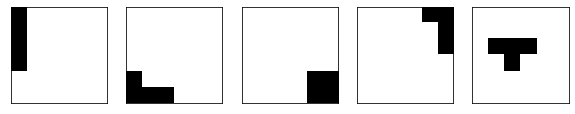
\includegraphics[width = 9.5cm]{figures/tetris.png}
    \caption{Basic tetris-like patterns}
    \label{fig::tetris}
  \end{subfigure}
  \begin{subfigure}[b]{\textwidth}
    \centering
    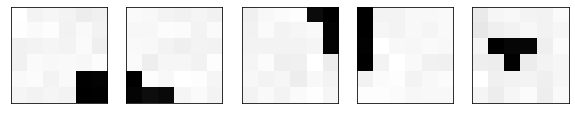
\includegraphics[width = 9.5cm]{figures/tetrisfeature.png}
    \caption{Features extracted from the data}
    \label{fig::tetrisfeature}
  \end{subfigure}
  \begin{subfigure}[b]{\textwidth}
    \centering
    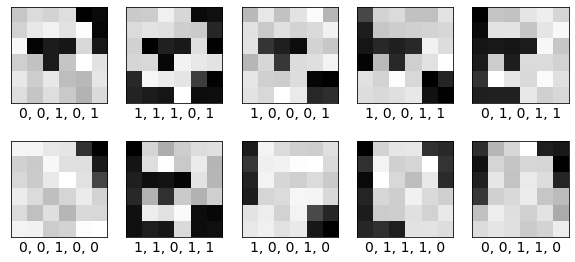
\includegraphics[width = 9.5cm]{figures/tetrisdetection.png}
    \caption{Features detected in images} 
    \label{fig::tetrisfeature}
  \end{subfigure}
  \caption{(b) Results of extracted features from the Gibbs sampler. These features perfectly coincide with the basic patterns, ignoring background noise. (c) Ten images are randomly selected and the labels correspond to latent features detected from the Gibbs sampler.}
\end{figure}

\begin{figure}[!h]
  \centering
  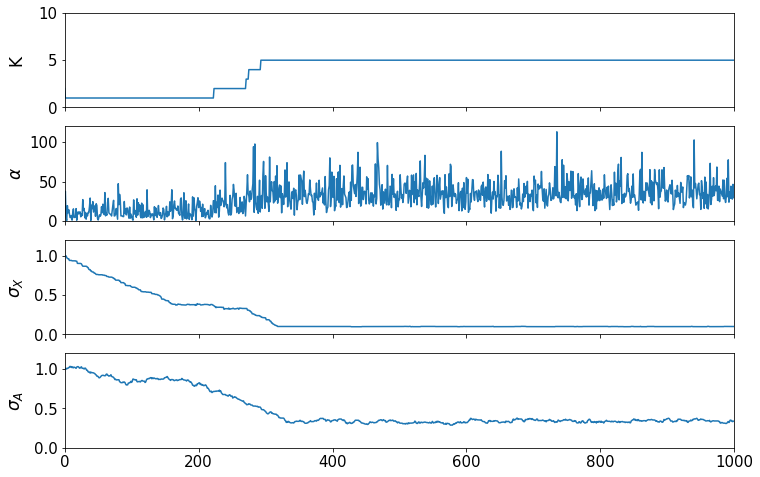
\includegraphics[width = \textwidth]{figures/gibbsresultblock.png}
  \caption{Trace plots for the dimensionality and parameters over $1000$ iterations of sampling. The posterior estimation of $\sigma_X = 0.0996$ is quite close to the true value $0.1$.}
  \label{fig::gibbsblock}
\end{figure}

\section{Simulation}\label{sec::simulation}

We performed a simulation study on a dataset of images generated from basic five tetris-like patterns (Fig \ref{fig::tetris}). Each image consists of one or multiple patterns and is disturbed by a random noise. Each pattern is embedded in a $6\times 6$ matrix which can be reshaped into a $36$-dimension vector. To elaborate it mathematically, let $\boldsymbol{f}_1, \cdots, \boldsymbol{f}_5$ represent the patterns in vector forms. The images $\{\boldsymbol{x}_{i}\}_{i=1}^N$ are independently generated by \begin{equation}\boldsymbol{x}_i = \sum_{j=1}^5 c_j \boldsymbol{f}_j + \boldsymbol{e}_i,\end{equation} where $c_j\in\{0,1\}$ are not all zero and $\boldsymbol{e}_i\sim\mathcal{N}(\boldsymbol{0}, 0.01 \mathbf{I})$.


The true value of $\sigma_X = 0.1$ under this setting. The parameters are initialized with $\sigma_X = \sigma_A = \alpha = 1$ and updated via Monte Carlo and Metropolis steps. The Gibbs sampler went through 1000 iterations, and stabilized in approximately $400$ iterations (Fig \ref{fig::gibbsblock}). The algorithm found $5$ latent features which perfectly indicated the presence and absence of the five patterns.

\section{Latent features in poker card images}\label{sec::realdata}

We applied this Gibbs sampler on a dataset consisting of $1056\times 691$ pixel PNG images of poker cards. We selected out 100 images from the suit of diamonds excluding Jack, Queen and King, cropped and downsampled each image to $80\times 44$ pixels in grayscale. We represented each image $\boldsymbol{x}_i$ by a flattened vector of $3520$ dimensions. An example of an original image and the corresponding processed image is shown in Fig \ref{fig::sample}. The Gibbs sampler was initialized with $\sigma_X = 0.15$, $\sigma_A = 0.25$ and $\alpha = 1$, and stabilized after approximately 100 iterations. We extracted the mean image in observance of the zero-mean prior on the features, and $14$ other latent features were suggested (Fig \ref{fig::gibbs}). The latent features, along with the reconstructed images are shown in Fig \ref{fig::featuremap}. 

\begin{figure}[!h]
  \centering
  \begin{subfigure}[b]{0.35\textwidth}
    \centering
    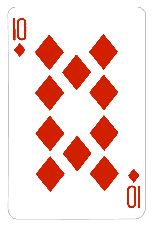
\includegraphics[width = 2.75cm]{figures/sample_original.png}
    \caption{Original image}
  \end{subfigure} 
  \begin{subfigure}[b]{0.35\textwidth}
    \centering
    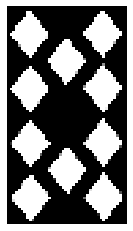
\includegraphics[width = 2.3cm]{figures/sample_cropped.png}
    \caption{Processed image}
  \end{subfigure}
  \caption{The original and processed image of ten of diamonds (10$\blacklozenge$)}
  \label{fig::sample}
\end{figure}

\begin{figure}[!h]
  \centering
  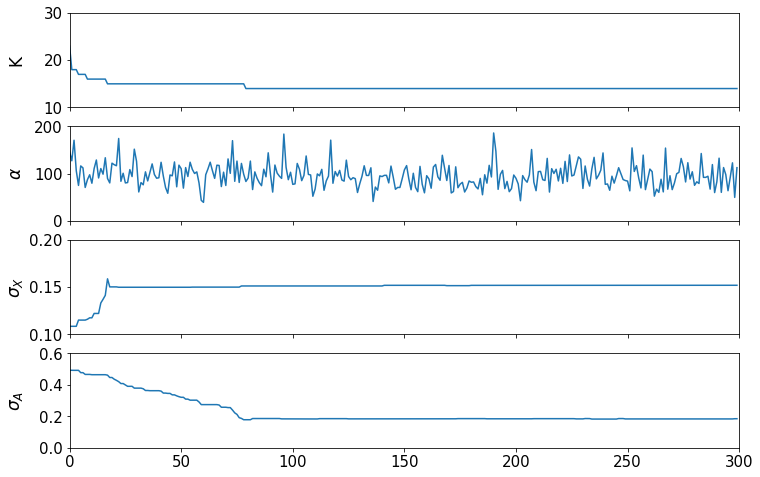
\includegraphics[width = \textwidth]{figures/gibbsresult.png}
  \caption{Trace plots for the dimensionality and parameters over $300$ iterations of sampling.}
  \label{fig::gibbs}
\end{figure}

\begin{figure}[!h]
  \centering
  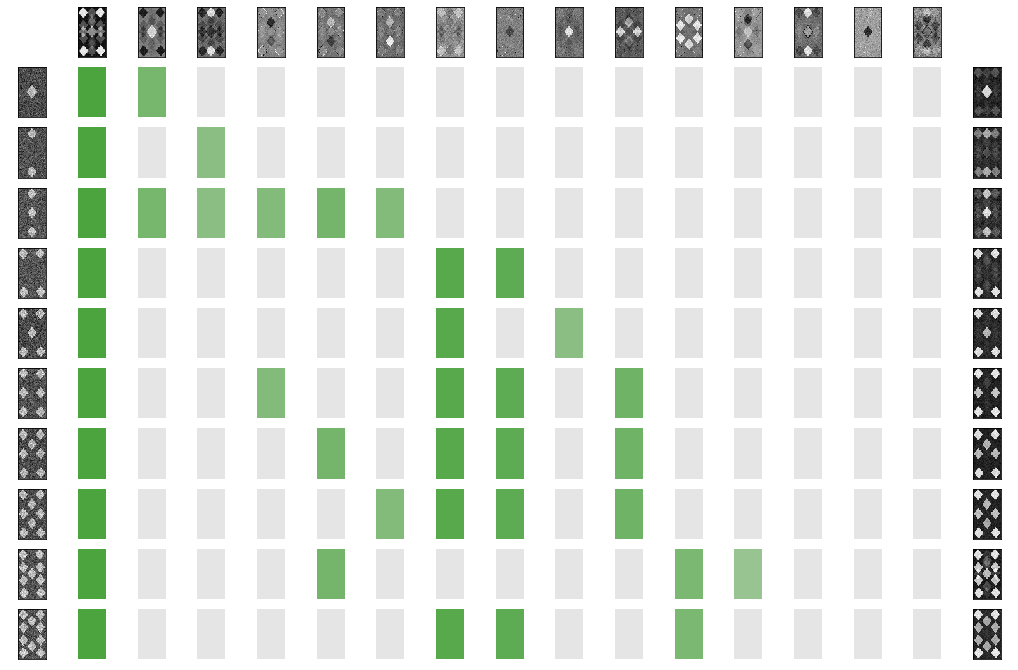
\includegraphics[width = \textwidth]{figures/featuremap.png} 
  \caption{Feature matrix in the left-ordered form. The mean image (left) and $14$ features are shown on the top. In the left-most column are the images for the first suit of cards, and the images reconstructed from the features are displayed on the right respectively. The rectangles in the middle indicate which features are possessed by the images, with colored rectangles showing possession and the gray ones showing non-possession. The shades of color indicate the frequency of that feature being possessed. Both indicators and the reconstructed images are based upon the 300th sample.}
  \label{fig::featuremap}
\end{figure}

Although it is hard to interprete all these latent features, it is delighting to see that the features are able to capture the symmetry in most card images and reveal some particular patterns. For example, feature 1 (excluding the mean image) captures the pattern of a diamond in the center (light) with no diamonds in the corners (dark), which is shared by A$\blacklozenge$ and 3$\blacklozenge$. It is also interesting to note some enhancing-declining pairs in these features. Feature 7 and 8 have opposite effects, as a dark diamond in the center removes it from 4$\blacklozenge$ and a light one enhances it on 5$\blacklozenge$. Similarly goes for feature 3 through 5. These features demonstrate a pattern of two diamonds vertically arranged in the middle. Feature 3 declines both diamonds while feature 5 enhances them. Feature 4, which has both a light and a dark diamond, enhances the one on the top and declines the other at the bottom. These features contribute to the difference among 6$\blacklozenge$, 7$\blacklozenge$ and 8$\blacklozenge$.



\section{Comparative Analysis}\label{sec::comparison}
Feature extraction, which involves reducing the dimensionality of original data, plays a significant role in data analysis. Through feature extraction, data in high dimensionality are embedded into a low dimension space while still being described with sufficient accuracy. Many feature extraction techniques have been proposed, from traditional methods on low-rank matrix approximation (e.g. PCA) to neural network based algorithms (e.g. autoencoder). A majority of these methods, however, requires predetermined hyperparameters controlling the number of features. On the poker card dataset, principal component analysis (PCA) requires 49 features to maintain information akin to our method (measured in variance). Although as few as $8$ components are sufficient to reconstruct the images with differences imperceptable to human eyes, determination on this number requires domain knowledge. Our methods extracted $14$ features without manual selection, which is slightly more redundant than $8$. However, it outperforms much over $49$ features suggested by PCA comparably in absence of manual selection.

Some other implementations can be found on the same algorithm as introduced in this paper, one of which is given by \citet{chai}. The authors of that implementation was able to reduce the running time by utilizing the one-rank update of matrix inversion \citep{griffiths2005infinite}, they failed to exploit sufficiently for potential speedup possibility. Furthermore, the code was not written in OOP (object oriented programming), nor was it well wrapped for reproduction.

The execution time of these implementations was recorded respectively under the same dataset. The profiling information is given in Table \ref{tbl::cmp}.

\begin{table}[!h]
  \centering
  \small
  \caption{Profile on simulated data introduced in Section \ref{sec::simulation}}
  \label{tbl::cmp}
  \begin{tabular}{lrrrrrr}
    \toprule
    & \multicolumn{3}{c}{Implementation of \citet{chai}} & \multicolumn{3}{c}{Our implementation} \\
    & \multicolumn{1}{c}{Total time}& \multicolumn{1}{c}{\# Exec} & \multicolumn{1}{c}{Avg. time} & \multicolumn{1}{c}{Total time}& \multicolumn{1}{c}{\# Exec} & \multicolumn{1}{c}{Avg. time} \\
    & \multicolumn{1}{c}{\scriptsize(sec)} & \multicolumn{1}{c}{} & \multicolumn{1}{c}{\scriptsize($\mu$sec)} & \multicolumn{1}{c}{\scriptsize(sec)} & \multicolumn{1}{c}{} & \multicolumn{1}{c}{\scriptsize($\mu$sec)} \\
    \midrule
    Sample $\mathbf{Z}$ & 450.754 & 970,000 & 464.694 & 140.783 & 490,218 & 287.184 \\
    Sample $K$ & 82.614 & 97,000 & 851.690 & 21.080 & 97,000 & 217.319 \\
    Sample $\alpha$ & 0.140 & 1,000 & 139.871 & 0.028 & 1,000 & 28.423\\
    Sample $\sigma_X$ & 0.348 & 1,000 & 347.566 & 0.248 & 1,000 & 248.225\\
    Sample $\sigma_A$ & 0.331 & 1,000 & 331.169 & 0.221 & 1,000 & 221.456\\
    Others & 2.386 & --------- & --------- & 1.821 & --------- & ---------\\
    Total & 536.572 & --------- & --------- & 164.182 & --------- & ---------\\
    \bottomrule
  \end{tabular}
\end{table}

\section{Discussion}\label{sec::discussion}
We have demonstrated that our implementation of the algorithm proposed by \citet{griffiths2005infinite} achieved satisfactory accuracy and efficiency. Also, we applied the algorithm on datasets where the observations are exchangeable and each observation possesses a finite subset of infinite latent features, and obtained reasonable and interpretable results. The strategy of taking the limit of a finite model from latent classes to infinite features provides a direction for a wild class of latent structures, such as in \citet{teh2006hierarchical} and \citet{chen2011hierarchical}.

Although the algorithm we implemented upon extended the models from definite latent classes to a set of latent features, limiting $\mathbf{Z}$ within the class of binary matrices may not be appropriate for many datasets. This constraint can be relaxed by allowing $\mathbf{Z}$ to take on natural numbers (count of features) or real numbers (proportion of features). Furthermore, the model is sensitive to location and scale. Identical patterns appearing in various position and size are not considered the same feature, which entangles its application in object detection or pattern recognition. Further work can be done on the improvement of the algorithm.

\bibliographystyle{plainnat}
\bibliography{ref}

\newpage
\begin{appendices}
  \section{The Indian buffet process}\label{sec::IBP}
  The Indian buffet process is a metaphor of Indian restaurant which generates a probability distribution on equivalence classes of binary matrices. Assume that the restaurant offers a buffet with infinite number of dishes, and a finite number $N$ of customers enter this restaurant sequentially. Each customer $i$ moves along the buffet and samples each dish $k$ with a probability of $m_k/i$, where $m_k$ is the number of previous customers who have sampled that dish. Then, the $i$-th customer tries a number of new dishes, randomly drawn from a Possion$(\alpha / i)$ distribution. The indicator matrix, the $(i,j)$-th entry showing whether the customer $i$ chose dish $j$, is a binary matrix from that distribution. It deserves attention that the distribution generated from Indian buffet process is actually exchangeable, although the customers enter in a certain order, because the numbering of the dishes can be arbitrarily permutated.

  The algorithm for sampling from the Indian buffet process is provided in Algorithm \ref{tbl::IBP}.
 
  \begin{algorithm}
    \caption{Sampling scheme from an Indian buffet process}
    \label{tbl::IBP}
    \KwIn{The number of rows $N$, parameter $\alpha$}
    \KwOut{A binary matrix $\mathbf{Z}$}
    Initialize $\mathbf{Z} = \mathbf{0}_{N\times 0}$, $\boldsymbol{c} = []$, $n = 0$\;
    \For{$i$ in permutated rows of $\mathbf{Z}$}{
      $n$++\;
      \For{$j$ in columns of $\mathbf{Z}$}{
        $u$ = sample $\mathbf{Z}[i,j]$ with probability $\boldsymbol{c}[j]/n$\;
        \If{$u == 1$}{
          $\boldsymbol{c}[j]$++\;
        }
        $k$ = sample from Possion$(\alpha/n)$\;
        append $\boldsymbol{c}$ with $k$ $1$'s\;
        right-append $\mathbf{Z}$ with $k$ columns with row $i$ being all $1$'s\;
      }

    }
  \end{algorithm}

  \section{Auxillary proofs}
  \subsection{Proof of calculating the conditional likelihood}\label{app::proof1}
    Assume $\mathbf{Z}$ is an $M\times K$ matrix and $M\gg K$. Denote $\lambda = \sigma_X^2 / \sigma_A^2$.
    Let $\mathbf{Z} = \mathbf{U}\mathbf{D}\mathbf{V}^\mathrm{T}$ be the singular value decomposition of $\mathbf{Z}$, where $\mathbf{D} = \mathrm{diag}\{d_1,\cdots, d_K\}$. 

    \begin{equation}
    \begin{aligned}
      \mathbf{Z}^\mathrm{T}\mathbf{Z} + \lambda \mathbf{I} &= \mathbf{V}\mathbf{D}^2 \mathbf{V}^\mathrm{T} + \lambda \mathbf{I} \\
      &= \mathbf{V} (\mathbf{D}^2 + \lambda \mathbf{I}) \mathbf{V}^\mathrm{T}.
    \end{aligned}
  \end{equation}
    Therefore, $|{\mathbf{Z}}^{\mathrm{T}}\mathbf{Z} + \lambda \mathbf{I}| = |\mathbf{D}^2 + \lambda \mathbf{I}| = \prod_{k=1}^K (d_k^2 + \lambda)$, and
    \begin{equation}
    \begin{aligned}
      \mathrm{tr}\left( \mathbf{X}^\mathrm{T} \left(\mathbf{I} -  \mathbf{Z} \left(\mathbf{Z}^\mathrm{T}\mathbf{Z} + \lambda \mathbf{I} \right)^{-1} \mathbf{Z}^\mathrm{T} \right) \mathbf{X} \right) &= \mathrm{tr}\left( {\mathbf{X}}^{\mathrm{T}} \mathbf{X}\right) - \mathrm{tr}\left( \mathbf{X}^\mathrm{T}\mathbf{U}\mathbf{\Lambda}\mathbf{U}^\mathrm{T}\mathbf{X} \right),
    \end{aligned}
  \end{equation}
    where $\mathbf{\Lambda} = \mathrm{diag}\{d_k^2/(d_k^2 + \lambda), k = 1,\cdots, K\}$. 
    The second term can be efficiently calculated. \begin{equation}
    \begin{aligned}
      \mathrm{tr}(\mathbf{X}^\mathrm{T}\mathbf{U}\mathbf{\Lambda}\mathbf{U}^\mathrm{T}\mathbf{X}) &= \mathrm{tr}\left(\sum_{k = 1}^K \frac{d_k^2}{d_k^2 + \lambda}{\mathbf{X}}^{\mathrm{T}}\boldsymbol{u}_{\cdot k}\boldsymbol{u}_{\cdot k}^\mathrm{T}\mathbf{X}\right) \\
      &= \sum_{k=1}^K \frac{d_k^2}{d_k^2 + \lambda}\boldsymbol{u}_{\cdot k}^\mathrm{T}\mathbf{X}{\mathbf{X}}^{\mathrm{T}}\boldsymbol{u}_{\cdot k}\\ 
      &= \sum_{k=1}^K \frac{d_k^2}{d_k^2 + \lambda}||{\mathbf{X}}^{\mathrm{T}}\boldsymbol{u}_{\cdot k}||_2^2.
    \end{aligned}
  \end{equation}
  \subsection{Proof of sampling $K_i^\text{new}$}\label{app::proof2}
    \begin{equation}
    \begin{aligned}
      \widetilde{\mathbf{W}} = {\widetilde{\mathbf{Z}}}^{\mathrm{T}}\widetilde{\mathbf{Z}} + \lambda \mathbf{I} &= \begin{bmatrix}
        {\mathbf{Z}}^{\mathrm{T}} \\ {\boldsymbol{e}}_i^{\mathrm{T}}
      \end{bmatrix} \begin{bmatrix}
        \mathbf{Z} & \boldsymbol{e}_i
      \end{bmatrix} = 
      \begin{bmatrix}
        \mathbf{W} & \boldsymbol{z}_{i \cdot} \\
        {\boldsymbol{z}}_{\cdot i}^{\mathrm{T}} & 1 + \lambda
      \end{bmatrix}.
    \end{aligned}
  \end{equation}
    By elementary transform of block matrix, 
    \begin{equation}
      \begin{bmatrix}
      \mathbf{I} & \boldsymbol{0} \\ -{\boldsymbol{z}}_{\cdot i}^{\mathrm{T}} \mathbf{W}^{-1} & 1
    \end{bmatrix}\widetilde{\mathbf{W}}
    \begin{bmatrix}
      \mathbf{I} & -\mathbf{W}^{-1}{\boldsymbol{z}}_{\cdot i}  \\ \boldsymbol{0}^\mathrm{T} & 1
    \end{bmatrix} = \begin{bmatrix}
      \mathbf{W} & \boldsymbol{0} \\ {\boldsymbol{0}}^{\mathrm{T}} & 1 + \lambda - {\boldsymbol{z}}_{\cdot i}^{\mathrm{T}} \mathbf{W}^{-1}{\boldsymbol{z}}_{\cdot i}
    \end{bmatrix}.
    \label{eqn::elemblocktrans}
    \end{equation}
    Note that ${\boldsymbol{z}}_{\cdot i}^{\mathrm{T}} \mathbf{W}^{-1}{\boldsymbol{z}}_{\cdot i} = \gamma_{ii}$, and let $\mu = 1 + \lambda - \gamma_{ii}$, we have
    \begin{equation}\log |\widetilde{\mathbf{W}}| - \log|\mathbf{W}| = \log \mu.\end{equation}
    It can be shown as well from (\ref{eqn::elemblocktrans}) that 
    \begin{equation}\begin{aligned}
      \widetilde{\mathbf{W}}^{-1} &= \begin{bmatrix}
      \mathbf{I} & -\mathbf{W}^{-1}{\boldsymbol{z}}_{\cdot i}  \\ \boldsymbol{0}^\mathrm{T} & 1
    \end{bmatrix}\begin{bmatrix}
      \mathbf{W}^{-1} & \boldsymbol{0} \\ {\boldsymbol{0}}^{\mathrm{T}} & \mu^{-1}
    \end{bmatrix}\begin{bmatrix}
      \mathbf{I} & \boldsymbol{0} \\ -{\boldsymbol{z}}_{\cdot i}^{\mathrm{T}} \mathbf{W}^{-1} & 1
    \end{bmatrix} \\
    &= \begin{bmatrix}
      \mathbf{W}^{-1} + \mu^{-1}\mathbf{W}^{-1}\boldsymbol{z}_{i \cdot}{\boldsymbol{z}}_{\cdot i}^{\mathrm{T}}\mathbf{W}^{-1} & -\mu^{-1}\mathbf{W}^{-1}\boldsymbol{z}_{i \cdot} \\
      -\mu^{-1}\boldsymbol{z}_{i \cdot}^\mathrm{T}\mathbf{W}^{-1} & \mu^{-1}
    \end{bmatrix}.
    \end{aligned}\end{equation}
    Hence, \begin{equation}
    \begin{aligned}
      \widetilde{\mathbf{\Gamma}} &= \begin{bmatrix}
        \mathbf{Z} & \boldsymbol{e}_i
      \end{bmatrix}\widetilde{\mathbf{W}}^{-1}\begin{bmatrix}
        {\mathbf{Z}}^{\mathrm{T}} \\ {\boldsymbol{e}}_i^{\mathrm{T}}
      \end{bmatrix} \\
      &= \mathbf{Z}(\mathbf{W}^{-1} + \mu^{-1}\mathbf{W}^{-1}\boldsymbol{z}_{i \cdot}{\boldsymbol{z}}_{\cdot i}^{\mathrm{T}}\mathbf{W}^{-1}){\mathbf{Z}}^{\mathrm{T}} - \mu^{-1}\boldsymbol{e}_i \boldsymbol{z}_{i \cdot}^\mathrm{T}\mathbf{W}^{-1}{\mathbf{Z}}^{\mathrm{T}} - \mu^{-1}\mathbf{Z}\mathbf{W}^{-1}\boldsymbol{z}_{i \cdot}\boldsymbol{e}_i^\mathrm{T} + \boldsymbol{e}_i {\boldsymbol{e}}^{\mathrm{T}} \\
      &= \mathbf{\Gamma} + \mu^{-1}(\boldsymbol{\gamma}_{\cdot i}\boldsymbol{\gamma}_{\cdot i}^\mathrm{T} - \boldsymbol{e}_i\boldsymbol{\gamma}_{\cdot i}^\mathrm{T} - \boldsymbol{\gamma}_{\cdot i}{\boldsymbol{e}}_i^{\mathrm{T}} + \boldsymbol{e}_i {\boldsymbol{e}}_i^{\mathrm{T}}) \\
      &= \mathbf{\Gamma} + \mu^{-1}(\boldsymbol{\gamma}_{\cdot i} - \boldsymbol{e}_i)(\boldsymbol{\gamma}_{\cdot i} - \boldsymbol{e}_i)^\mathrm{T}.
      \label{eqn::gammaupdate}
    \end{aligned}
  \end{equation}
    Therefore, the trace can be updated via \begin{equation}
    \begin{aligned}
      \widetilde{t} - t &= \mathrm{tr}({\mathbf{X}}^{\mathrm{T}}(\mathbf{I} - \widetilde{\mathbf{\Gamma}})\mathbf{X}) - \mathrm{tr}({\mathbf{X}}^{\mathrm{T}}(\mathbf{I} - \mathbf{\Gamma})\mathbf{X}) \\
      &= \mathrm{tr}({\mathbf{X}}^{\mathrm{T}}(\mathbf{\Gamma} - \widetilde{\mathbf{\Gamma}})\mathbf{X}) \\
      &= -\mu^{-1}\mathrm{tr}({\mathbf{X}}^{\mathrm{T}}(\boldsymbol{\gamma}_{\cdot i} - \boldsymbol{e}_i)(\boldsymbol{\gamma}_{\cdot i} - \boldsymbol{e}_i)^\mathrm{T}\mathbf{X}) \\
      &= -\mu^{-1}||{\mathbf{X}}^{\mathrm{T}}(\boldsymbol{\gamma}_{\cdot i} - \boldsymbol{e}_i)||_2^2.
    \end{aligned}
  \end{equation}
    It is worthwhile to notice that to do not need calculating $\mathbf{W}$ and $\mathbf{\Gamma}$, as we do not care about constant terms in posterior probability. What we actually need is the ratio \begin{equation}\frac{p(\mathbf{X}\mid \mathbf{Z}_{i,k}^{+},\sigma_X,\sigma_A)P(K_i^\text{new} = k\mid\alpha)}{p(\mathbf{X}\mid \mathbf{Z},\sigma_X,\sigma_A)P(K_i^\text{new} = 0\mid\alpha)} = \prod_{j = 0}^{k-1} \frac{p(\mathbf{X}\mid \mathbf{Z}_{i,j+1}^{+},\sigma_X,\sigma_A)P(K_i^\text{new} = j+1\mid\alpha)}{p(\mathbf{X}\mid \mathbf{Z}_{i,j}^{+},\sigma_X,\sigma_A)P(K_i^\text{new} = j\mid\alpha)},\end{equation}
  or equivalently \begin{multline}\log p(\mathbf{X}\mid \mathbf{Z}_{i,j+1}^{+},\sigma_X,\sigma_A) - \log p(\mathbf{X}\mid \mathbf{Z}_{i,j}^{+},\sigma_X,\sigma_A) \\+ \log P(K_i^\text{new} = j+1\mid\alpha) - \log P(K_i^\text{new} = j\mid\alpha)
  \label{eqn::logdiff}
  \end{multline}
    for $j = 0, 1,\cdots, k-1$.
    In a recursive scheme, we can always view $\mathbf{Z}_{i,j}^+$ as baseline and $\mathbf{Z}_{i, j+1}^+$ is exactly adding a column $\boldsymbol{e}_i$ on the right of $\mathbf{Z}_{i,j}^+$.

    Using the notations above, (\ref{eqn::logdiff}) can be evaluated as \begin{equation}D\log \left(\frac{\sigma_X}{\sigma_A}\right) - \frac{D}{2}\log \mu + \frac{1}{2\sigma_X^2}\mu^{-1}||{\mathbf{X}}^{\mathrm{T}}(\boldsymbol{\gamma}_{\cdot i} - \boldsymbol{e}_i)||_2^2.\end{equation}

    Recall that $\mu = 1 + \lambda - \gamma_{ii}$ which can be obtained from $\boldsymbol{\gamma}_{\cdot i}$. It suffices to show that $\widetilde{\boldsymbol{\gamma}}_{\cdot i}$ can be updated directly through $\boldsymbol{\gamma}_{\cdot i}$.
    It immediately follows (\ref{eqn::gammaupdate}) that \begin{equation}\widetilde{\boldsymbol{\gamma}}_{\cdot i} = \boldsymbol{\gamma}_{\cdot i} + \mu^{-1}(\gamma_{ii} - 1)(\boldsymbol{\gamma}_{\cdot i} - \boldsymbol{e}_i).\end{equation}
  \section{Package Installation}
      The implemented package, \textbf{IBPILFM}\citep{bolin}, can be downloaded and installed via \texttt{pip}.
      \vspace{0.3cm}
      \shellcmd{pip install -i https://test.pypi.org/simple/ IBPILFM\vspace{0.3cm}}
      To upgrade, run following codes in terminal. (The latest version is \texttt{0.1a4} as for Apr 30, 2020.)
      \vspace{0.3cm}
      \shellcmd{pip install -{}-upgrade -i https://test.pypi.org/simple/ IBPILFM\vspace{0.3cm}}
      You can check the status of installation via
      \vspace{0.3cm}
      \shellcmd{python\vspace{0.3cm}}
      and in python interactive shell, run
      \vspace{0.3cm}
      \pythoncmd{import ibp\\>{}>{}>{} ibp.\_\_version\_\_\vspace{0.3cm}}
      The package is successfully installed if version is displayed (e.g. \texttt{'ibp-0.1a4'}).

  \section{Collaborators}
      
      \textbf{Bo Liu}, Master's in Statistical Science, Duke University.
      \begin{itemize}[leftmargin = 7mm]
        \item[--] Author of the package
        \item[--] Mathematical derivations
        \item[--] Example on poker cards 
        \item[--] Report writeup 
      \end{itemize}

      \textbf{Linlin Li}, Master's in Statistical Science, Duke University.
      \begin{itemize}[leftmargin = 7mm]
        \item[--] Co-author of the package
        \item[--] Unit tests
        \item[--] Example on Tetris blocks
        \item[--] Package maintenance 
      \end{itemize}
\end{appendices}

\end{document}
